\chapter{Solarzelle und Halbleiterdiode}
\label{v:17}

Anhand der Charakteristiken von Halbleiterdioden und Solarzellen soll diese weit verbreitete Technologie näher gebracht werden.

%------------------------------------------------
\section{Stichworte}
%------------------------------------------------

Halbleiterdiode; Kennlinie einer Diode; Kennlinie einer Solarzelle (SZ), Arbeitspunkt (MPP) der SZ, Spektrale Empfindlichkeit der SZ; Farbe von Licht.
%
%------------------------------------------------
\section{Literatur}
%------------------------------------------------

Gehrtsen, Kapitel 11.1.2, 11.2.10, 11.3 und 14.4.3
%
%------------------------------------------------
\section{Anwendungsbeispiele}
%------------------------------------------------

Die Sonne ist die Hauptenergiequelle für unser tägliches Leben. Dabei kann diese Energie vor sehr langer Zeit geliefert worden sein, wie bei den fossilen Brennstoffen, indirekt, wie bei Windkraftwerken oder direkt, wie bei Sonnenkollektoren und Solarzellen. Solarzellen sind in Reihe geschaltete photoempfindlichen Halbleiterdioden, die zur Stromerzeugung genutzt werden. Die Spannung entsteht dabei durch optische Anregung von Valenzelektronen in das Leitungsband. Die mögliche Leistung, die eine Solarzelle zu erbringen vermag hängt dabei von der Beleuchtungsstärke und Farbe des beleuchtenden Lichtes ab. Im Versuch werden die physikalischen und elektrischen Eigenschaften von Halbleiterdioden studiert und die Energieerzeugung mit Hilfe einer Solarzelle quantitativ untersucht.

%------------------------------------------------
\section{Theoretischer Hintergrund}
%------------------------------------------------

\subsection{Halbleiter}

Durch die Anordnung im Kristallgitter verschieben sich die Energieniveaus der Siliziumatome ein klein wenig gegeneinander. Das führt dazu, daß die Niveaus in sogenannten Bändern nahe beieinanderliegen. Dasjenige Band, in dem sich die am schwächsten gebundenen Elektronen (Valenzelektronen) befinden, nennt man das \textit{Valenzband}. \\
Dieses ist durch eine \textit{Bandlücke}, in der es keine erlaubten Energieniveaus gibt, vom nächsthöheren Band getrennt. Da unter normalen Bedingungen keine Elektronen Zustände in diesem Band besetzen und die Energieniveaus benachbarter Atome energetisch sehr dicht aneinander liegen, kann ein Elektron, welches durch äußere Anregung in dieses Band gelangt, sich quasi-frei durch den Kristall bewegen und damit zur elektrischen Leitung beitragen. Daher bezeichnet man dieses Band als \textit{Leitungsband}.

\subsubsection{Dotierung}

Man kann in einen reinen Kristall aus vierwertigem Silizium bei der Herstellung Fremdatome einbringen, um die elektrische Charakteristik des Materials zu verändern. Dieser Prozess heißt \textit{Dotierung}.\\
Bringt man dreiwertige Atome in den Kristall (\textit{Akzeptor}, typischerweise Bor), so bleibt eine der Kristallbindungen zu den vier Nachbaratomen unvollständig, da ein Elektron für die kovalente Bindung fehlt. Diese unvollständige Bindung absorbiert leicht Elektronen aus dem Leitungsband, was ein fehlendes Elektron an einer anderen Stelle hinterläßt, da der Kristall insgesamt elektrisch neutral ist. Da auch diese neue, unvollständige Bindung leicht ein Elektron absorbiert, kann man dieses ''fehlende'' Elektron im Kristall als beweglich ansehen, es verhält sich also wie eine freie, positive Ladung. Man bezeichnet diese als \textit{Loch} im Valenzband. Auf diese Weise reichert eine Bor-Dotierung den Halbleiter mit positiven Ladungsträgern an, man nennt den Kristall auch \textit{p-dotiert}.\\
Auf dieselbe Weise führt Dotierung mit einem fünfwertigen Element (\textit{Donator}, typischerweise Phosphor) zu einem Überschuß an negativen Ladungsträgern, der Kristall ist \textit{n-dotiert}.

\subsection{$pn$-Diode}

Beim idealen $pn$-\"Ubergang grenzen zwei gleichm\"assig dotierte $p$-
und $n$-dotierte Schichten aneinander. Durch die unterschiedliche
Konzentration freier Ladungstr\"ager auf beiden Seiten kommt es zur
Diffusion: Elektronen des $n$-dotierten Gebiets wandern zur
$p$-dortierten Seite und k\"onnen dort mit L\"ochern rekombinieren. Die 
ortsfesten Atome, die ja nun ionisiert sind, stellen eine
positive {\it Raumladung} dar. Analog wandern L\"ocher aus der
$p$- in die $n$-Zone und rekombinieren. Eine negative Raumladung
entsteht.\\
Diese Raumladungen erzeugen ein elektrisches Feld,
welches der Diffusion entgegenwirkt und zu einem Gleichgewicht
f\"uhrt. Die Spannung, welche durch das elektrische Feld erzeugt
wird, nennt man {\it Diffusionsspannung}, $U_{\mathrm{D}}$. Das Gebiet
um den $pn$-\"Ubergang, welches frei von beweglichen Ladungstr{\"a}gern
 ist, wird {\it Verarmungszone} genannt. 
Die Ausdehnung der Verarmungszone auf die
jeweilige Seite ist proportional zum inversen der
Ladungstr\"agerkonzentration.

\subsubsection{$pn$-\"Ubergang mit \"ausserer Spannung in Durchlaßrichtung}

Legt man an den $pn$-\"Ubergang eine externe Spannung an, so dass die
Anode an die $p$-Schicht und die Kathode an die $n$-Schicht
angeschlossen ist, werden die Elektronen aus dem $n$-Gebiet zum
$p$-Gebiet hin verschoben und andersherum. Die angelegte Spannung,
$U_{\mathrm{F}}$, wirkt der Diffusionsspannung entgegen. Es gilt f\"ur
die Potentialdifferenz am $pn$-\"Ubergang:
%
\begin{equation}
U_{pn} = U_{\mathrm{D}} - U_{\mathrm{F}} \, .
\end{equation}

\noindent
Mit zunehmender externer Spannung w\"achst der Strom durch den
$pn$-\"Ubergang. Man spricht von einem {\it Durchlassstrom}.

\subsubsection{$pn$-\"Ubergang mit \"ausserer Spannung in Sperrrichtung}

Legt man eine externe Spannung mit umgekehrter Polung,
$U_{\mathrm{R}}$, an den $pn$-\"Ubergang, so verst\"arkt diese die
Diffusionsspannung und man erh\"alt
%
\begin{equation}
U_{pn} = U_{\mathrm{D}} + U_{\mathrm{R}} \, .
\end{equation}

Die Elektronen der $n$-Schicht und die L\"ocher der $p$-Schicht werden
von der Verarmungszone weggezogen. Die Verarmungszone w\"achst. Da
kein Strom fließen kann wird diese Art der Beschaltung auch {\it
Sperrrichtung} genannt.

\begin{figure}[ht!]
\begin{center}
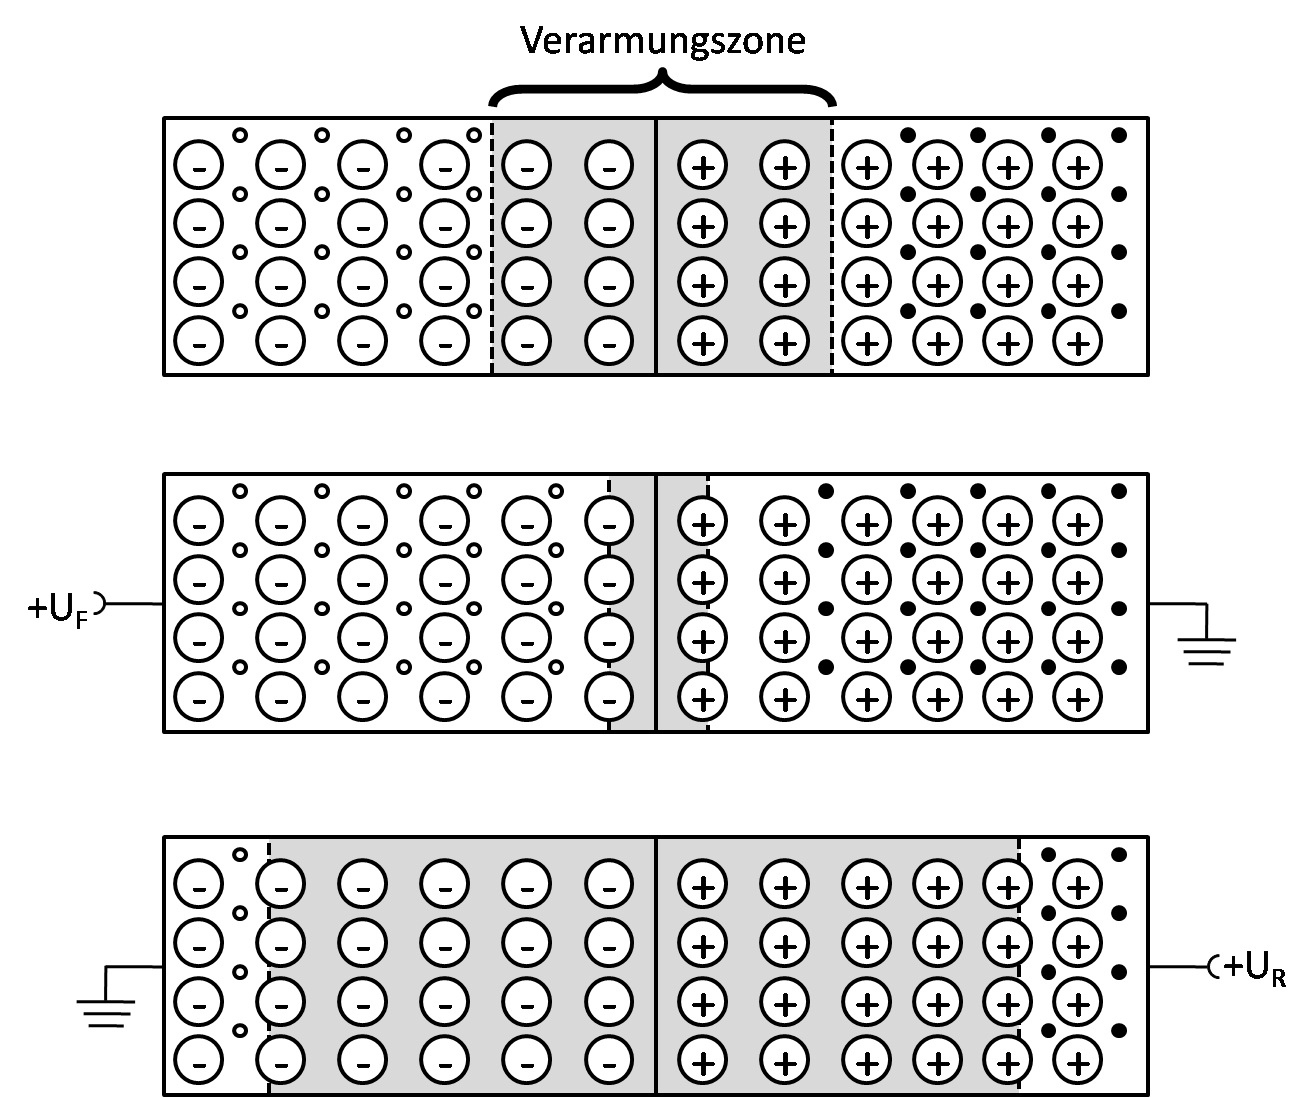
\includegraphics[width=0.45\textwidth]{Versuch_17-18/Abbildungen/pn_Uebergang.jpg}
\end{center}
\caption{$pn$-\"Ubergang ohne angelegte Spannung (oben), mit \"ausserer Spannung in Durchlaß- (Mitte) und Sperrrichtung (unten).}
\label{fig:Verarmung}
\end{figure}

\subsubsection{Durchbruch}

Im Sperrbetrieb k\"onnen hohe elektrische Felder in der Sperrschicht
auftreten. Durch den {\it Lawineneneffekt} kommt
es zu einem starken Anstieg des {\it Sperrstroms}. Diesen Effekt bezeichnet 
man als {\it Durchbruch} des $pn$-\"Ubergangs.\\

\noindent
\textbf{Lawineneffekt.} 
%
Elektronen, welche durch thermische Anregung in der Sperrschicht entstehen,
werden durch das elektrische Feld beschleunigt. Bei ausreichender
Energie k\"onnen Elektronen aus Atomverb\"anden herausgeschlagen
werden. Diese sekund\"aren Elektronen k\"onnen ihrerseits durch
St\"osse Atome ionisieren und sorgen damit f\"ur einen ansteigenden
Strom.

\subsection{Ladungsdeposition in der verarmten Diode}

Geladene Teilchen (Elektronen, Myon, etc.) und Licht (Photonen) geben über verschiedene Prozesse Energie ab, wenn sie durch ein Material fliegen. Beim Halbleiter erzeugt diese Energie durch Ionisation Paare von Elektronen und Löchern, welche sich im Kristall frei bewegen können. Im elektrischen Feld, welches in der Verarmungszone herrscht, werden diese Ladungen zu den Elektroden hin beschleunigt und erzeugen so einen Strom durch die Diode und den außen angeschlossenen Stromkreis.\\
Je nach den benutzten Materialien der Diode, ihrer Dicke und der Anzahl an Teilchen oder Photonen, die die Diode pro Sekunde treffen, kann dieser Strom groß genug werden, um technisch genutzt werden zu können. Das ist das Prinzip der Solarzelle.

\subsection{Solarzellen}

Man kann sich eine Solarzelle als aus einer Stromquelle und einer Diode zusammengesetzt vorstellen. Dabei hängt die Stromstärke von der Beleuchtung ab. Wenn man die Solarzelle verdunkelt, dann misst man die Kennlinie einer Diode. Die Kennlinie einer beleuchteten Solarzelle ist daher lediglich um den Kurzschlussstrom $I_k$ nach unten verschoben (siehe Abbildung unten).\\ %\ref{fig:Kennlinienfeld}).\\
\begin{figure}[h]
	\centering
		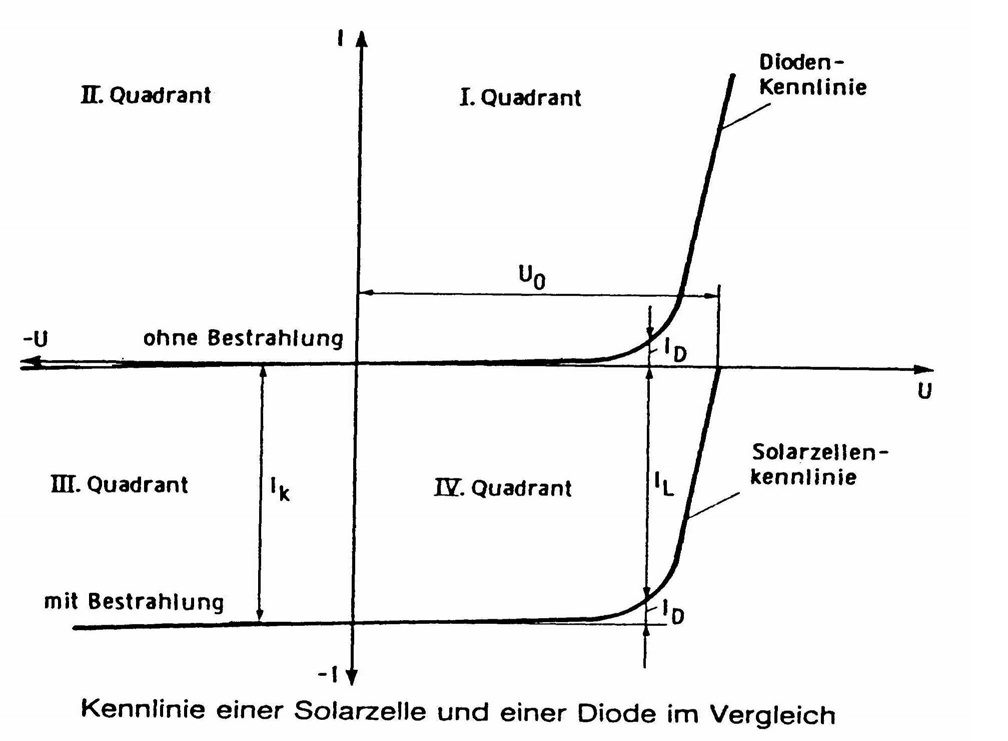
\includegraphics[width=0.5\textwidth]{Versuch_17-18/Abbildungen/Kennlinienfeld.jpg}
	\label{fig:Kennlinienfeld}
\end{figure}

Da bei Beleuchtung der Solarzelle in der Regel nur der vierte Quadrant der Darstellung interessiert, wird auch nur dieser gezeichnet. Trägt man die abgegebene Leistung $P$ über der Spannung auf, kann man ein Maximum ablesen, das als Maximum Power Point bezeichnet wird (siehe Abbildung nächste Seite).\\ %\ref{fig:Leistung}).\\
Schaltet man Solarzellen in Serie, addieren sich die Spannungen, während sich der Strom nicht ändert. Bei Parallelschaltung addieren sich dagegen die Ströme, wobei die Spannung erhalten bleibt. Solarzellen werden daher zu leistungsfähigen Modulen zusammen geschaltet.\\
Im Versuch wird ein in aus 19 Einzelelementen geschaltetes Solarmodul verwendet.

\begin{figure}[h]
	\centering
		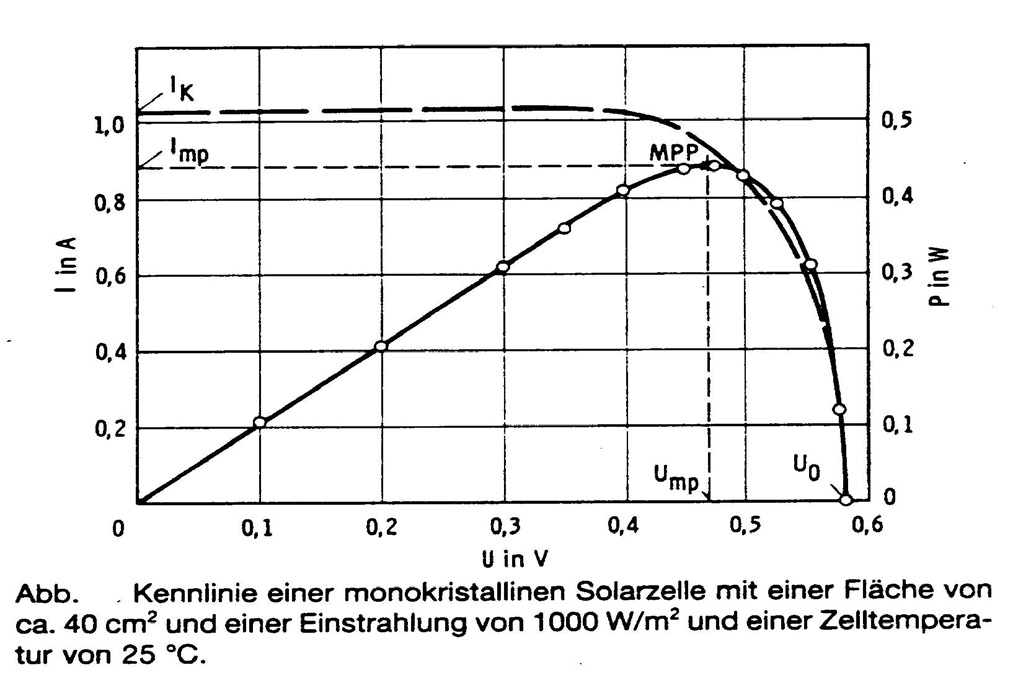
\includegraphics[width=0.5\textwidth]{Versuch_17-18/Abbildungen/Leistung.jpg}
	\label{fig:Leistung}
\end{figure}

%------------------------------------------------
\section{Fragen zur Vorbereitung}
%------------------------------------------------

\begin{enumerate}
	%
	%\item Was soll heute im Praktikum gemessen werden? Warum?
	%
	\item Was sind Valenz- und Leitungsband eines elektrischen Leiters?
	%
	\item Wie schaltet man ein Volt- oder Amperemeter in einen elektrischen Schaltkreis?
	%
	\item Was ist die Energielücke zwischen Valenz- und Leitungsband?
	%
	\item Was versteht man unter Löchern im Valenzband? Wie tragen sie zum Ladungstransport bei?
	%
	\item Was versteht man unter der Dotierung eines Halbleiters? Nennen Sie ein Beispiel!
	%
	\item Was sind Akzeptor- / Donatorniveaus im Bändermodell eines Halbleiters? Wie wirken sie auf die Energielücke im Halbleiter?
	%
	\item Was passiert beim Zusammenbringen eines p- und eines n-dotierten Halbleiters mit den freien Ladungsträgern?
	%
	\item Was ist die Diffusionsspannung (auch Diodenflussspannung)?
	%
	\item Was bedeutet Schaltung in Sperr- / Flussrichtung?
	%
	\item Wie sieht die I(U)-Kennlinie der Diode aus? %Was ist die Antidiffusionsspannung?
	%
	\item Was ist eine Solarzelle? Wie erzeugt sie eine elektrische Spannung (Stichwort: Elektronen-Loch-Paar Erzeugung)?
	%
	\item Wie sieht die I(U)-Kennlinie einer Solarzelle im Vergleich zu einer gewöhnlichen Diodenkennlinie aus? Wie unterscheiden sie sich?
	%
	\item Was ist der Maximal Power Point im P(U)-Diagramm einer Solarzelle?
	%
\end{enumerate}

%------------------------------------------------
\section{Durchführung} 
%------------------------------------------------

\begin{figure}[h]
	\centering
		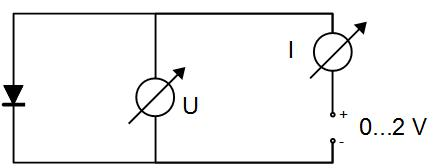
\includegraphics[width=0.5\textwidth]{Versuch_17-18/Abbildungen/Schaltung_Kennlinie.jpg}
	\label{fig:Schaltung_Kennlinie}
	\caption{Schaltung zur Messung der Kennlinie der Halbleiterdiode.}
\end{figure}

\begin{enumerate}
	%
	\item \textbf{Die Kennlinie einer unbeleuchteten Halbleiterdiode:}\\
		Messen Sie die I(U)-Kennlinie der Diode im Bereich 0\,V - 0.4\,V in Schritten von 0.1\,V und im Bereich von 0.4 V\,- 0.8\,V in Schritten von 0.02\,V und bestimmen Sie daraus $U_F$.\\
		\begin{minipage}{0.6\textwidth}
		\textbf{Achtung: }\\
		Keine Spannung über 2\,V anlegen (Schalter auf der Versuchsbox)!\\
		Wenn die Überlastwarnleuchte aufleuchtet wird dies im Protokoll vermerkt und die Messung abgebrochen.\\
		Vor dem Einschalten den Assistenten fragen!
		\end{minipage}
		\begin{minipage}{0.4\textwidth}
			\includegraphics[width=0.8\textwidth]{Versuch_17-18/Abbildungen/Bild15.jpg}
			\label{fig:Bild15}
		\end{minipage}
	%
	\item \textbf{Die Kennlinie einer unbeleuchteten Solarzelle:}\\
		Ersetzen Sie die Diode durch das Solarmodul.\\
		Verdunkeln Sie die auf dem Abschirmgehäuse aufgesteckte Solarzelle mit einem der optischen Filter und messen Sie die I(U)-Kennlinie im Bereich von 0\,V bis etwa 10\,V in Schritten von 1\,V.
	%
 
	\begin{minipage}{0.6\textwidth}
			\item \textbf{Die Kennlinie einer beleuchteten Solarzelle:}\\
		Ersetzen Sie das Netzgerät durch den regelbaren Lastwiderstand und entfernen Sie den Filter.
	\end{minipage}
	\begin{minipage}{0.4\textwidth}
				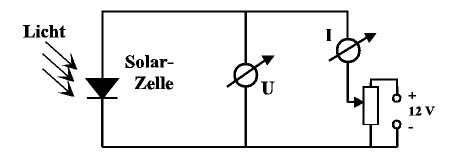
\includegraphics[width=1.00\textwidth]{Versuch_17-18/Abbildungen/solarzelle.jpg}
				\label{fig:solarzelle }
		\end{minipage}
	%
	\item \textbf{Die Kennlinien einer spektral gefiltert beleuchteten Solarzelle:}\\
		Setzen sie nacheinander die verschiedenen Spektralfilter in das Abschirmgehäuse ein. Nehmen Sie die Kennlinien für blaues, grünes und gelbes Licht von 0\,V bis 5\,V in 1\,V-Schritten, darüber hinaus in 0.2\,V-Schritten auf.
\end{enumerate}

%------------------------------------------------
\section{Auswertung} 
%------------------------------------------------

Die Diodenkennlinie lässt sich für kleinere Ströme annäherungsweise durch die Schottky-Gleichung beschreiben:
\begin{equation}
I = I_{Sp}\cdot\left(\exp\left(\frac{eU}{kT}\right)-1\right)
\end{equation}
Dabei ist $I_{Sp}$ der Sperrstrom, $e$ die Elementarladung, $k$ die Boltzmannkonstante, $T$ die absolute Temperatur (in Kelvin gemessen) und $U$ die Spannung, die über Anode und Kathode der Diode anliegt. Die Diodenflussspannung $U_F$ entspricht dem Schnittpunkt der U-Achse mit der Geraden, durch die man den steil ansteigenden Teil der Diodenkennlinie im Durchlassbereich approximiert.

\begin{enumerate}
	%
	\item Zeichnen Sie die $I(U)$-Kennlinien der Halbleiterdiode und bestimmen Sie aus der Auftragung graphisch die Diodenflussspannung $U_F$ mit Fehler!
	%
	\item Zeichnen Sie die $I(U)$-Kennlinien der unbeleuchteten Solarzelle und bestimmen Sie aus der Auftragung graphisch die Diodenflussspannung $U_F$ mit Fehler!
	%
	\item Tragen Sie die $I(U)$-Kennlinien aus Versuchsteil 3 und 4 auf und bestimmen Sie daraus den Kurzschlussstrom $I_k$ sowie die Leerlaufspannung $U_L = U (I = 0)$. Dazu müssen Sie gegebenenfalls den Graphen extrapolieren. 	
		Auch diese Größen sind mit Fehler behaftet, schätzen Sie diesen daher grob ab!
	%
	\item Bestimmen Sie die von der Solarzelle abgegebenen Leistungen $P = U \cdot I$ für die vier mit Beleuchtung gemessenen Kennlinien und tragen Sie diese in einen Graphen über der Spannung $U$ auf. Aus den Graphen wird der Maximal Power Point abgelesen $(P_{max}$, $I(P_{max})$ und $U(P_{max}))$. Berechnen Sie den Fehler mithilfe der Fehlerfortpflanzung. Sie können davon ausgehen, daß die Messgerätegenauigkeit bei 1\% des Messwertes liegt.
	%
	\item Die spektrale Empfindlichkeit $S$ der Solarzelle soll überprüft werden. Dazu wird das Verhältnis der spektralen Empfindlichkeiten bei gelbem (Wellenlänge $\lambda$ = 670\,nm) und grünem (Wellenlänge $\lambda$ = 530\,nm)
		Licht gebildet und mit dem Literaturwert (siehe Diagramm: \textit{Empfindlichkeit gegen Wellenlänge einer Photodiode}) für dieses Verhältnis verglichen.
		\begin{equation}
			\frac{S_{Gelb}}{S_{Gruen}}=\frac{\frac{I_K(Gelb)}{P_{Lampe}(Gelb)}}{\frac{I_k(Gruen)}{P_{Lampe}(Gruen)}}
		\end{equation}
		Hier sind $I_k$ die Kurzschlussströme der Solarzelle für die verschiedenen Filter, $P_{Lampe}$ ist die Strahlungsleistung der Lampe.
\end{enumerate}
Beim verwendeten Aufbau ist die Strahlungsleistung der Lampe mit dem gelben Filter $P_{Lampe}(Gelb)$ um 10\% größer als bei Verwendung des grünen Filters ($P_{Lampe}(Gruen)$). Daher benötigen Sie nicht die absolute Leistung der Glühlampe.

\noindent
Da die Intensität des Sonnenlichts bei etwa 880\,nm maximal ist, baut man Solarzellen so, dass sie in diesem Bereich ihre maximale Empfindlichkeit haben. Je weiter man sich von diesem Maximum entfernt, umso geringer wird auch die Empfindlichkeit (Messung 3).

\begin{minipage}{0.5\textwidth}
	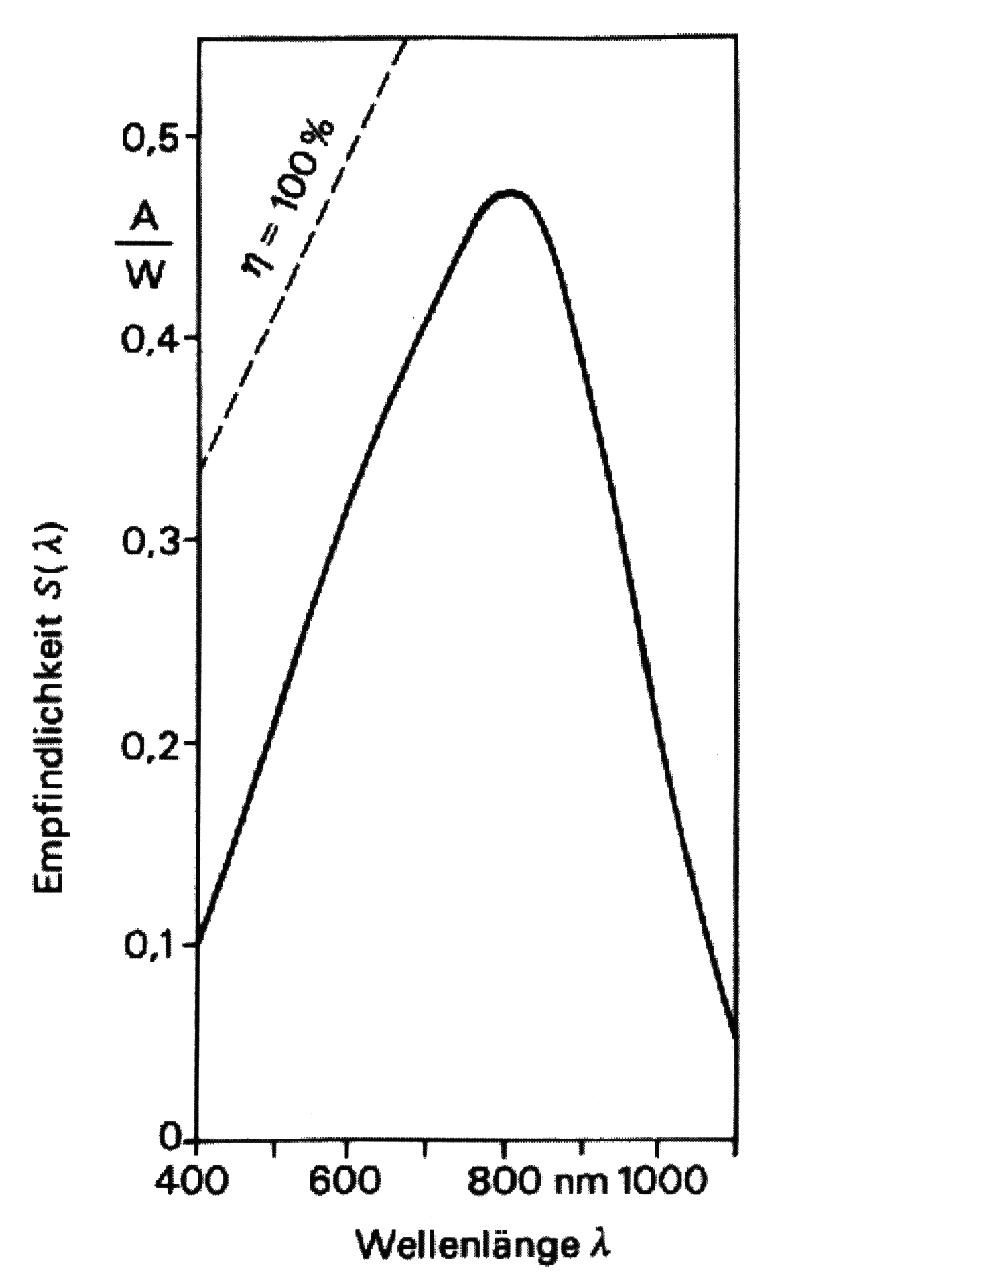
\includegraphics[width=1.00\textwidth]{Versuch_17-18/Abbildungen/QE_Solarzelle.JPG}
	\label{fig:BILD17}
\end{minipage}
\begin{minipage}{0.5\textwidth}
Das nebenstehende Bild zeigt die Empfindlichkeit einer Si-Photo-Diode in Abhängigkeit von der Wellenlänge. Gestrichelt eingezeichnet ist der Verlauf der Empfindlichkeit einer idealen Diode mit einer Ausbeute von 100\%.
Die gemessene Kurve liegt generell tiefer, verläuft aber bei kurzen Wellenlängen etwa parallel zur theoretischen Kurve.
Der steile Abfall auf der langwelligen Seite kommt daher, dass die Photonen nicht mehr genügend Energie haben, um Elektronen über die Bandlücke anzuregen.
\end{minipage}